% Author: Izaak Neutelings (December 2022)
\documentclass[border=3pt,tikz]{standalone}
\usepackage{physics}
\usepackage{siunitx}
\usepackage{graphicx}
\usetikzlibrary{angles,quotes} % for pic (angle labels)
\tikzset{>=latex}

\begin{document}

% ADD LABELS
\begin{tikzpicture}[x=1cm,y=1cm]
  
  % MAIN FIGURE
  \def\w{21.19cm} % width fine-tuned to match grid
  \node[inner sep=0,outer sep=0,above right] at (-0.0469*\w,-0.0584*\w) {
    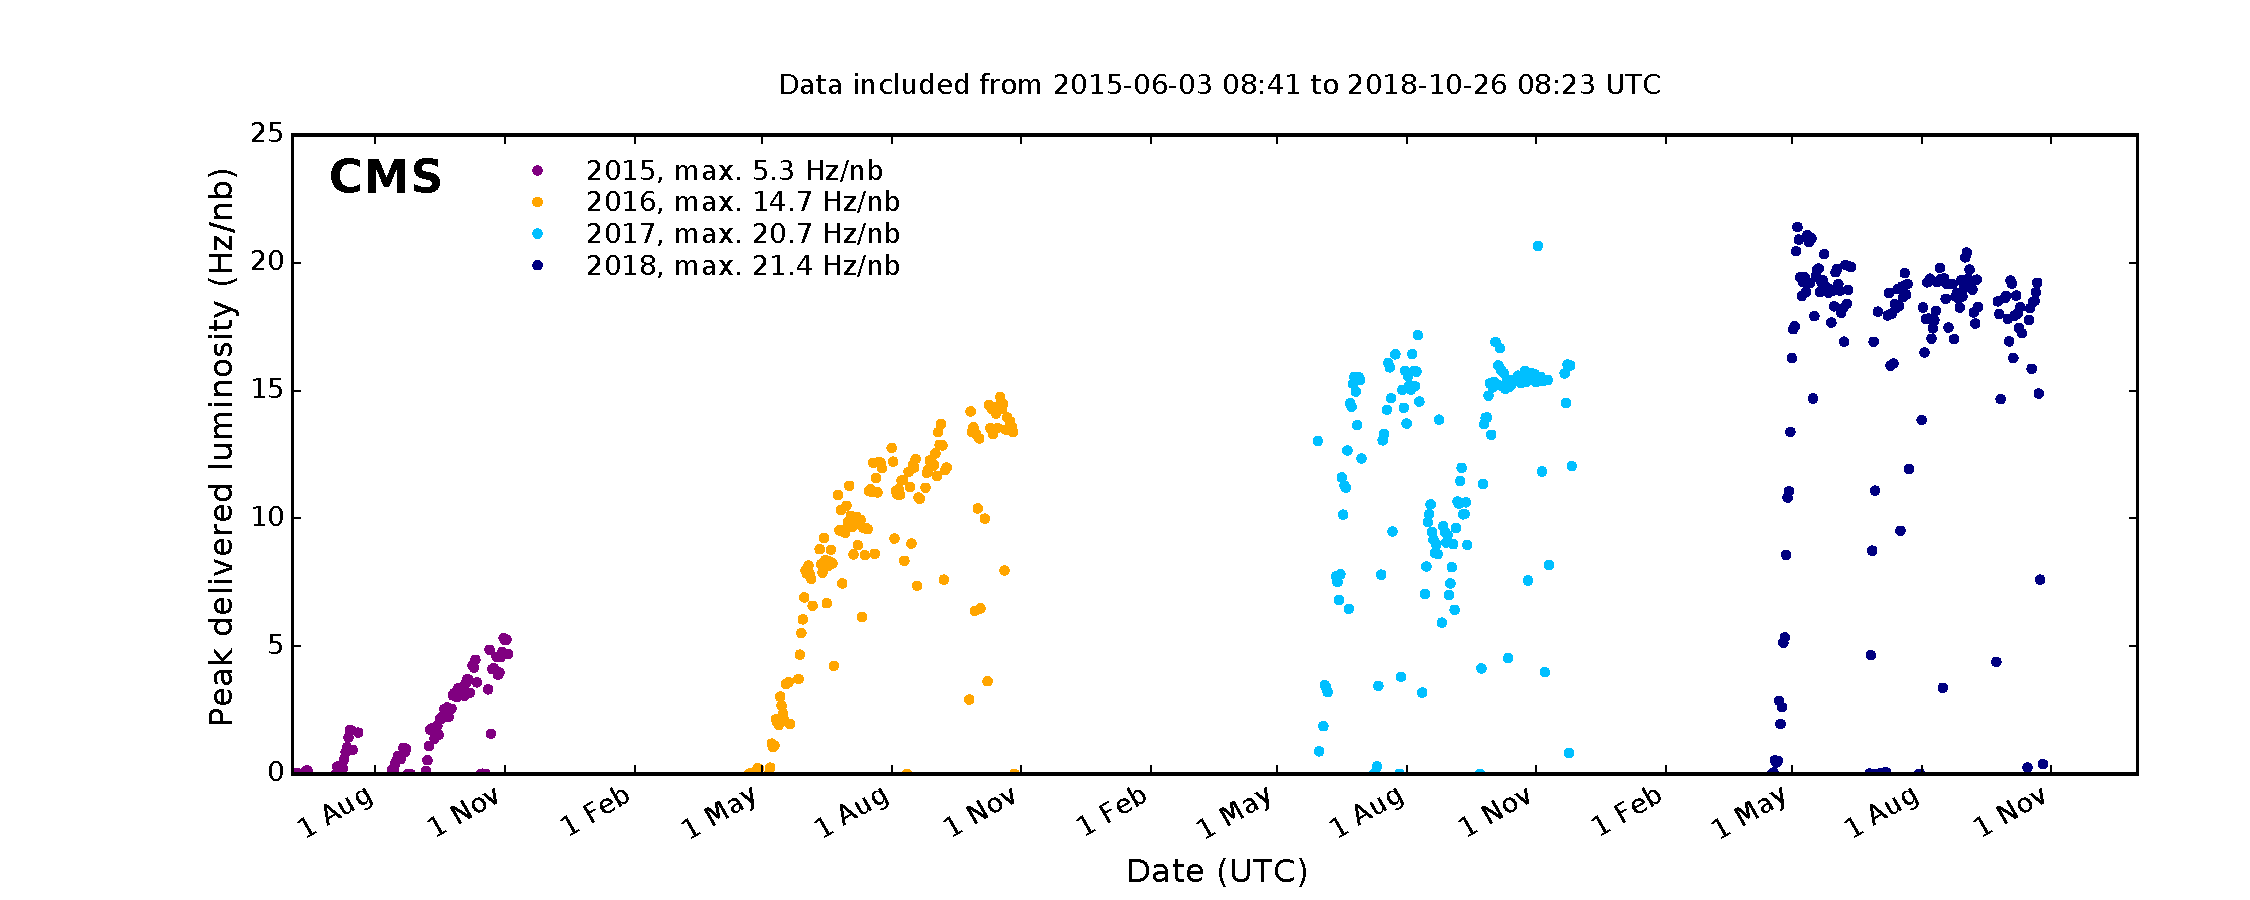
\includegraphics[width=\w,clip,trim={34mm 2mm 16mm 10mm}]{CMS_luminosity_peak_Run2.pdf}
  };
  
  %% HELP GRID
  %\draw[red,very thin,dashed] (0,0) grid[step=1cm] (20,7);
  %\draw[red,very thin] (0,0) grid[step=2cm] (20,7);
  %\fill[red!80!black] (0,0) circle(0.5mm);
  
  \def\designlumi{2.7715} % design lumi
  \draw[red!90!black,line width=0.8] (0.011,\designlumi) -- (19.99,\designlumi)
    node[pos=0.05,above right=0,inner sep=1pt,scale=0.9]
    {$\mathcal{L}^\text{design}_\text{peak} = \SI{1e34}{cm^{-2}s^{-1}}$};
  %\draw[red!90!black,line width=0.8] (0.011,2*\designlumi) -- (19.99,2*\designlumi)
  %  node[pos=0.5,above=0,inner sep=1pt,scale=0.9]
  %  {$\mathcal{L}_\text{peak} = \SI{2e34}{cm^{-2}s^{-1}}$};
  \draw[black,line width=0.33] (0.0,\designlumi) --++ (0.0905,0);
  \draw[black,line width=0.33] (20.0,\designlumi) --++ (-0.089,0);
  %\draw[black,line width=0.33] (0.0,2*\designlumi) --++ (0.0905,0);
  %\draw[black,line width=0.33] (20.0,2*\designlumi) --++ (-0.089,0);
  
\end{tikzpicture}

\end{document}
